\documentclass{ufsctex/ufsctex}
\usepackage{graphics}
\usepackage{graphicx}
\usepackage{enumitem}
\usepackage{float}
\usepackage[cache=false]{minted}
\usepackage{pgfplots}
\usepackage{smartdiagram}
\usepackage{tikz}
\usetikzlibrary{shapes,decorations,arrows}
\tikzstyle{block} = [rectangle, draw, fill=blue!20, text width=5em, text centered, rounded corners, minimum height=4em]
\tikzstyle{oval} = [draw, ellipse,fill=red!20, node distance=3cm, minimum height=2em]
\title{Estudo sobre o uso da linguagem GraphQL na composição de dados através de serviços baseados em JSON}
\begin{document}
\instituicao[a]{Universidade Federal de Santa Catarina}
\departamento[o]{Departamento de Informática e Estatística}
\curso[o]{Programa de Graduação em Sistemas de Informação}
\documento[o]{{Trabalho de Conclusão de Curso}}
\titulo{Estudo sobre o uso da linguagem GraphQL na composição de dados através de serviços baseados em JSON}
\autor{Mateus Maso}
\grau{Bacharel em Sistemas de Informação}
\local{Florianópolis, SC}
\data{\today}
\orientador{Prof. Dr. Frank Augusto Siqueira}

\capa
\folhaderosto

% \epigrafe{
  Time has told me not to ask for more,
  someday our ocean will find its shore
} {(Nick Drake)}

\paginaepigrafe

\textoResumo{  
  Para acomodar a rápida transformação na demanda de dados por clientes de aplicações distribuídas, tem se discutido cada vez mais novas e eficientes formas de disponibilizar estruturas de dados em serviços para consumo de clientes. Contudo, as atuais formas de comunicação cliente-servidor tem deixado o lado do cliente dependente da implementação do fluxo de dados e estilo de arquitetura oferecida pela API do servidor. Isso porque clientes precisam se preocupar em escrever código voltado ao acesso direto de estruturas de dados, levando a um acoplamento de API muitas vezes indesejado. Para evitar isso, este trabalho realiza um estudo sobre o uso da linguagem GraphQL como solução no desenvolvimento de uma ferramenta para que clientes possam buscar e compor estruturas de dados JSON através de serviços sem a necessidade de entender interfaces de aplicação. Permitindo que equipes de desenvolvimento possam constantemente questionar, experimentar e realizar mudanças no fluxo de dados de API's com o objetivo de diminuir o tempo de resposta e tamanho de dados sem ter impacto no código dos clientes.
}
\palavrasChave{
  GraphQL,
  REST,
  JSON Schema.
}

\paginaresumo
\begin{resumo}[Abstract]
  \begin{otherlanguage*}{english}
    In order to keep pace with the increasing changes on data queries executions by client over Web APIs, services have been applying efforts to fine-tune interface methods to maintain efficient client-server communication. However, there are services difficulties in managing changes in the API because, depending on the data fetching code implemented by the clients that access them, there is the possibility of compromising much of the communication. In order to develop solutions for the coupling problem, this work performs a study on the usage of GraphQL language and API description formats to propose a client-server communication model through automation in the execution of data queries. Thus, the model aims to guide client developers to the implementation of data fetching codes independent on API specification. As a result, a tool foresaw by the model is developed to validate its applicability. \\ \\
    \textbf{Key-words}: GraphQL. REST. JSON Hyper-Schema.
  \end{otherlanguage*}
\end{resumo}

\listadefiguras
\listadetabelas
\listadesimbolos

\simbolo{AST}{Árvore sintática abstrata}
\simbolo{API}{Interface de Programação de Aplicação}




\sumario
% % Introdução

\chapter{INTRODUÇÃO}

As orientações aqui apresentadas
são baseadas em um conjunto de normas
elaboradas pela ABNT.
Além das normas técnicas a
Biblioteca também elaborou uma série de tutoriais
e guias que estão disponíveis na sua Homepage.
\url{http://portalbu.ufsc.br/normalizacao-de-trabalhos-2/}.

\section{OBJETIVOS}

Descrição...

\subsection{Objetivo Geral}

Descrição...

\subsection{Objetivos Específicos}

Descrição...

# Introdução

- O crescimento das “API’s”
	- Estatisticas sobre o mercado
		- numeros sobre crescimento
		- numeros sobre distribuiçao de estilos
		- numeros sobre projeções futuras
	- Por que ocorreu isso?
		- SOA is the way to go
		- “dev is shifting more and more to the client.”
		- companies want get faster into new platforms.
	- Qual problema isso está causando?
		- Clientes dependentes de tipos/estilos de serviço
	- Por que isso é ruim?
		- (Perf) Estilos de API podem estar sendo sub/super utilizadas devido a constante mudança fluxo de dados em que clientes vivem.
		- (Inovação) Investir em novos modelos/tipos/estilos requer tempo para analisar o impacto no cliente.
		- (Agile) APIs tendem a crescer verticalmente e adicionar features em serviços “monoliticos” podem atrasar o crescimento de uma organização.
	- Como resolver isso?
		- Impedir que o cliente tenha acesso direto as APIs
	- De que forma?
		- Criar uma ferramenta intermediária responsável por transformar dependencias de entidades em requisições para os serviços.
	- Além disso, o que a ferramenta promove?
		- Experimentação, adoçao e composição de APIs
		- Desenvolvimento continuo no cliente
		- Documentação de API’s em formatos machine-readable
		- Despreocupação em entender o fluxo de dados
		- Aumentar tempo de resposta diminuindo o tráfego e dados.
		- Avisos sobre problemas e melhorias na comunicação.
		- Uso de microserviços ao invés de serviços monoliticos

  Its been slowly creeping up on us, creating exciting new possibilities for our applications; APIs are changing the face of the Web.

  The web has essentially become a service oriented platform, where information and functionality is a available through an API; the Web succeeded where the enterprise largely failed.

  This success can be attributed to the fact that the web has been decentralized in its approach and has adopted less stringent technologies to become service oriented. Many early APIs were written using SOAP but now REST is the dominant force (though some are more REST than others).  The publication of REST APIs has been rapidly increasing.

  Some offer both SOAP and REST APIs, but this practice has been on the decline and REST is now preferred for most new APIs.

  [How REST replaced SOAP on the Web: What it means to you]
  [http://www.infoq.com/articles/rest-soap]

\chapter{Fundamentos}

Neste capítulo são estabelecidos os principais conceitos utilizados ao longo do projeto. Será feito uma breve abordagem sobre os fundamentos de representação de dados; seguido pelo formato de serialização no qual será estudado e, por fim, tipos de serviços e tecnologias utilizadas para desenvolver a ferramenta.

\section[Serialização de Dados]{Serialização de Dados}

Na ciência da computação, serialização de dados é um processo de tradução usado para converter estruturas de dados\footnote{
  Uma estrutura de dados é uma forma abstrata de representar e organizar dados. Seu objetivo é ajudar a reduzir complexidade, podendo armazenar dados de diferentes tipos, como números, strings ou até mesmo outras estruturas de dados.
} em formatos que possam ser armazenados, transmitidos e reconstruídos por um mesmo ou outro ambiente computacional. \cite{Cline2016}

Dados serializados normalmente vivem mais tempo que suas aplicações de origem e, ao ser armazenado em disco ou transmitido pela rede, são representados de modo diferente que sua estrutura em memória. Para se ler dados serializados em memória é preciso realizar o processo inverso, também chamado de deserialização, onde estes passam a ser representados por estruturas da linguagem de execução. \cite{Guller2016}

\begin{figure}[H]
  \centering
  \includegraphics[width=\textwidth,height=\textheight,keepaspectratio]{figuras/data-serialization-deserialization.png}
  \caption{Processo de serialização e deserialização}
\end{figure}

Este processo, embora demande tempo, permitiu que aplicações fizessem o consumo de informações de forma distribuída, contribuindo com o aumento do volume de dados que circulam pela internet. Além disso, fez-se necessário a seleção adequada de formatos de serialização cuja estrutura não prejudique o desempenho de aplicações na busca por dados. \cite{SumarayMakki2012}

Segundo a Cisco Systems\footnote{
  Empresa de sistemas de rede.
}, de 2014 para o ano 2015, houve um aumento de 21\% no volume de tráfego de dados registrados apenas por seus aparelhos. Sendo a categoria Web, Email e Data responsável por representar aproximadamente 7,558 petabytes de dados transmitidos por seus clientes durante um mês. \cite{Cisco2016}

Para suprir esta alta demanda, diversos formatos de serialização foram introduzidos para melhor atender os problemas de desempenho experienciados por serviços. Dentre eles, tempo de serialização e deserialização, tamanho de transferência, flexibilidade de uso, facilidade de leitura, automação, suporte para linguagem, entre outros. \cite{Guller2016}

\begin{table}[ht!]
  \centering
  \resizebox{\columnwidth}{!}{
    \begin{tabular}{|c|c|c|c|c|}
      \hline
      Formato & Especificação & Codificação & Human-Readable & Esquema/IDL \\
      \hline
      XML & Padronizada & Textual & Sim & Sim \\ 		  
      \hline
      JSON & Padronizada & Textual & Sim & Parcial \\
      \hline
      YAML & Padronizada & Textual & Sim & Parcial \\
      \hline
      Avro & Padronizada & Binário & Não & Sim \\
      \hline
      Protocol Buffers & Padronizada & Binário & Parcial & Sim \\
      \hline
      Thrift & Não Padronizada & Binário & Parcial & Sim \\
      \hline
    \end{tabular}
  }
  \caption{Comparação de formatos de serialização}
\end{table}

Para melhor entender cada formato, será feito uma abordagem sobre algumas das categorias de classificação usadas para estudar o desempenho dos formatos existentes hoje.

\input{capitulos/fundamentos/serializacao-de-dados/especificacao/index}
\input{capitulos/fundamentos/serializacao-de-dados/codificacao/index}
\input{capitulos/fundamentos/serializacao-de-dados/human-readable/index}
\input{capitulos/fundamentos/serializacao-de-dados/esquema-idl/index}

\section{JSON}

JSON ou Javascript Object Notation é um formato de serialização de dados human-readable baseado em texto com especificação padronizada e parcialmente descritivo. Foi desenvolvido por Douglas Crockford com o objetivo de representar dados em uma maneira simples, leve e flexível através da redução na sobrecarga de marcações comparado ao formato XML.

Por ter se adaptado bem no ambiente de aplicações distribuídas, este formato acabou sendo amplamento utilizado por empresas como principal forma de represetação de dados serializados em seus serviços. A figura 2 mostra claramente a preferência do formato JSON por desenvolvedores ao criar novas APIs. \cite{Duvander2013}

\begin{figure}[H]
  \centering
  \resizebox{\columnwidth}{!}{
    \includegraphics[width=\textwidth,height=\textheight,keepaspectratio]{figuras/xml-vs-json.png}
  }
  \caption{Porcentagem de novas APIs em XML e JSON}
\end{figure}

Na sua essência, JSON foi construído com base em 4 tipos primitivos de dados e outros 2 para composição. Cada tipo possui seu respectivo correspondente na maioria das linguagens de programação, embora possam ser identificados por nomes diferentes. \cite{Droettboom2015}

\begin{table}[H]
  \centering
  \resizebox{\columnwidth}{!}{
    \begin{tabular}{|c|c|c|c|c|}
      \hline
      Tipo & Exemplo de Valor \\
      \hline
      Object & \mintinline{c}{ {"key1": "value1", "key2": "value2"} } \\
      Array & \mintinline{c}{ ["first", "second", "third"] } \\
      Number & \mintinline{c}{ 1, -1, 2.9999 } \\
      String & \mintinline{c}{ "This is a string" } \\
      Boolean & \mintinline{c}{ true, false } \\
      Null & \mintinline{c}{ null } \\
      \hline
    \end{tabular}
  }
  \caption{Exemplo de tipos de valores em JSON}
\end{table}

Através da composição de listas, objetos e tipos primitivos, é possível representar complexas estruturas de dados que aplicações possam vir a serializar. No entanto, não existe um único padrão de representação em JSON, uma vez que dado uma estrutura para serializar, é possível representá-lo de inúmeras maneiras. \cite{Droettboom2015}

Por exemplo, a seguir estão duas formas diferentes de representação em JSON para os mesmo dados de uma entidade “pessoa”:

\begin{figure}[H]
  \centering
  \inputminted[frame=single,framesep=10pt]{javascript}{anexos/pessoa.json}
  \caption{Primeiro exemplo de representação JSON}
\end{figure}

\begin{figure}[H]
  \centering
  \inputminted[frame=single,framesep=10pt]{javascript}{anexos/pessoa-2.json}
  \caption{Segundo exemplo de representação JSON}
\end{figure}

Ambas representações são válidas, apesar da figura 4 estar representando dados em uma estrutura mais formal que a outra. No entanto, por ser um formato não descritivo, a responsabilidade de entender o que está sendo representado em JSON vai depender da análise crítica ou conhecimento prévio dos desenvolvedores. Já uma máquina, sem conhecer o contexto, não saberia como interpretar os dados de forma correta. \cite{Droettboom2015}

Para isso, será abordado em seguida um dos formatos de descrição existentes hoje para descrever estruturas JSON utilizados no projeto.

\input{capitulos/fundamentos/json/json-schema/index}

\section{REST}

REST ou Representational State Transfer é um estilo de arquitetura usada para a comunicação de sistemas distribuídos através do protocolo HTTP. Foi introduzido por Roy Fielding em 2000 com o objetivo de oferecer às aplicações web um modelo de interface de acesso baseada em recursos. Além disso, descreve seis tipos de restrições que serviços deveriam aplicar para ganho de performance, escalabilidade, simplicidade, modificabilidade, visibilidade, portabilidade e confiabilidade.

Em virtude de causar grande repercussão após sua publicação, o termo REST, segundo Richardson, acabou sofrendo diversas interpretações durante o tempo e, sua descrição representada de formas não originalmente propostas por Fielding. Alguns descrevem que serviços que violam essas restrições não podem ser considerados RESTful. Para Wildermuth, apesar de reconhecer as vantagens de cada restrição, serviços web devem usá-los de forma pragmática. \cite{RichardsonEtAl2013} \cite{Wildermuth2015}

Ao ser introduzido no mercado de API's, REST acabou se adaptando bem por ter se mostrado uma solução de fácil acesso em clientes web, mobile apps e IoTs\footnote{
  Internet of Things
}. Segundo Pautasso, a eliminação da complexidade existente em Web Services antes de sua publicação em 2000 fez com que REST fosse considerado um dos principais responsáveis pela popularização de arquiteturas orientada a serviços. \cite{PautassoEtAl2008}

\begin{figure}[H]
  \centering    \includegraphics[width=0.9\textwidth,height=\textheight,keepaspectratio]{figuras/api-styles.jpg}
  \caption{Distribuição de estilos e protocolos para API's}
\end{figure}

A seguir será feita uma abordagem sobre os seis tipos de restrições propostas por Fielding, o que é o termo RESTful, além de entrar em detalhe sobre as atuais soluções para descrição de API's.

Esta seção fornece uma visão geral sobre as restrições propostas por Fielding para a implementação em arquiteturas web, além de ser examinado o impacto de cada restrição nesses sistemas distribuídos. \\

\textbf{Cliente-Servidor} \\

Nesta primeira restrição, não existe conexão entre cliente e servidor, mas sim a espera do servidor por pedidos de clientes através de chamada e resposta. O cliente (consumidor do serviço) não se preocupa com tarefas de comunicação de banco de dados, gerenciamento de cache, entre outros. Assim como o servidor (prestador de serviços) não está preocupado com as tarefas do cliente como interface ou experiência do usuário por exemplo. Permitindo a evolução independente dos dois ambientes, \textit{desde que sua interface de comunicação não seja alterada}. \cite{Fielding2000} \\

\textbf{Sem Estado} \\

Esta restrição ajuda na viabilidade, confiabilidade e escalabilidade de sistemas distribuídos, pois garantem que chamadas à API não estejam vinculadas a um determinado servidor. Como HTTP é um protocolo sem conexão, cada requisição deve conter todas as informações necessárias para que um servidor entenda o que um cliente está executando. Para Wildermuth, no entanto, dependendo da diversidade no número de clientes, ao manter um servidor sem estado, perder-se o controle no tamanho da estrutura de resposta necessária para atender a demanda de todos os clientes. \cite{Wildermuth2015} \\

\textbf{Interface Uniforme} \\

Em essência, Fielding propõe que aplicações façam o uso de verbos HTTP (POST, GET, PUT, DELETE) e identificadores uniforme de recursos (URI) para mapear operações em ambientes distribuidos e minimizar o acoplamento entre cliente-servidor. Essas regras de acesso são: \cite{Fielding2000}

\begin{itemize}[noitemsep]
\item Identificação de Recursos: Cada recurso deve ser disponibilizado através de uma URI específica e coesa. (Exemplo: GET /customers/1)
\item Manipulação de Recursos através de Representações: Um recurso pode ser representado em diferentes formatos para diferentes clientes. (Exemplo: HTML, XML, JSON)
\item Resposta Auto-explicativa: Metadados devem ser adicionados na requisição e resposta de um recurso para descrever seu estado atual ou desejado. (Exemplo: código de resposta HTTP, Host, Content-Type)
\item HATEOAS\footnote{
  Hypermedia as the Engine of Application State.
} - Caso um recurso possua relacionamentos, ao ser representado, estes devem estar especificados em forma de hiperlinks para facilitar a navegação de dados por clientes.
\end{itemize}

\textbf{Separação em Camadas} \\

Um dos princípios desta restrição está em evitar que clientes façam diretamente requisição para o servidor sem antes passar por um intermediário, como por exemplo um load balancer\footnote{
  Técnica para distribuir a carga de trabalho uniformemente entre dois ou mais computadores
}. Assegurando que clientes apenas se preocupem com a comunicação, deixando para que intermediários lidem com a distribuição de requisições. \cite{Fielding2000}

\begin{figure}[H]
  \centering  	   \includegraphics[width=0.6\textwidth,height=\textheight,keepaspectratio]{figuras/load-balancer.png}
  \caption{Exemplo de Load Balancer}
\end{figure}

\textbf{Código sob Demanda} \\

Apesar de ser a única restrição opcional do estilo, ela permite que servidores disponibilizem código em forma de script para que seja executado no cliente. Dessa forma, extendendo a lógica de serviço do servidor para seus clientes. \cite{Fielding2000} \\

\textbf{Cache} \\

Para aumentar desempenho de um serviço. Quando um recurso é acessado por mais de um cliente, se não houve mudança é recomendado que a resposta seja armazenada em cache, evitando o processamento desnecessário. Isso significa que servidores, quando possível, devem implementar regras de cache para beneficio de ambos os ambientes. \cite{Fielding2000}

\section{GraphQL}

GraphQL é uma linguagem de consulta de dados e interpretador de consultas para APIs. Foi desenvolvida pelo Facebook em 2012 mas sua especificação apenas publicada em 2015. Tem com objetivo fornecer uma descrição completa e compreensível de dados disponíveis em interfaces de aplicação. Além disso, permite que clientes façam consultas para busca exata de dados que desejam trabalhar. \cite{GraphQL2016}

Importante ressaltar que GraphQL não é uma linguagem para banco de dados, por mais que possa ser utilizado para esta finalidade. Ao invés, sua linguagem e interpretador trabalham com a idéia de mapeamento de campos e tipos de dados em aplicações, fornecendo uma interface unificada e amigável para desenvolvimento de produtos, além de uma plataforma poderosa para a construção de ferramentas. \cite{GraphQL2016}

Por ser uma especificação, GraphQL possui implementações em diversas linguagens de programação e atualmente é usado em diversos contextos, como comunicação entre cliente-servidor, microserviços, simplificação de APIs, navegação de árvores, gerador de consultas para banco de dados, entre outros.

Para gerar um esquema GraphQL, antes é preciso definir os tipos de estruturas, seus campos de acesso e funções para mapear e retornar dados reais em código.

\begin{figure}[H]
  \centering
  \inputminted[frame=single,framesep=10pt]{javascript}{anexos/pessoa.js}
  \caption{API de um código em JavaScript}
\end{figure}

\begin{figure}[H]
  \centering
  \inputminted[frame=single,framesep=10pt]{javascript}{anexos/pessoa-graphql-schema.graphql}
  \caption{Esquema GraphQL para API em JavaScript}
\end{figure}

Uma vez que o esquema GraphQL foi gerado, pode ser enviado consultas GraphQL para construção de estruturas de dados. Primeiramente, é feito a validação da consulta para garantir que esta só se refere aos tipos e campos definidos, em seguida, executa as funções fornecidas para produzir um resultado. \cite{GraphQL2016}

\begin{figure}[H]
  \centering
  \inputminted[frame=single,framesep=10pt]{javascript}{anexos/pessoa-graphql-query.graphql}
  \caption{Query GraphQL para esquema}
\end{figure}

\begin{figure}[H]
  \centering
  \inputminted[frame=single,framesep=10pt]{javascript}{anexos/pessoa-graphql-query-response.json}
  \caption{Resposta JSON da Query GraphQL}
\end{figure}

\input{capitulos/fundamentos/graphql/linguagem-de-consulta/index}
\input{capitulos/fundamentos/graphql/sistema-de-tipagem/index}
\input{capitulos/fundamentos/graphql/introspeccao/index}


% \chapter{Desenvolvimento}

Dizer que os últimos 2 capítulos foram pra contextualizar os conceitos utilizados no projeto desenvolvido. Dizer que nos próximos subcapítulos são descritos o processo de planejamento de projeto, detalhes de implementação da ferramenta e a etapa de validação, com foco no impacto da ferramenta no processo de mudança no fluxo de dados pelo servidor.

\section{Planejamento de Projeto}

% Explicar protótipo (flow de execução) e usar diagramas para melhor visualizar/entender. Entrar apenas em detalhes importantes de implementação como redução de AST, algoritmo de ordenação de prioridade e geraçao de requests. Abordar os testes pra validação, objetivo deles, o que será analisado e o que precisa ser desenvolvido pra poder rodar no ambiente sugerido.

\begin{enumerate}
\item Como evitar quebrar clientes na mudança de fluxo de dados?
\item Descrever execution flow
\item Como mapear recursos de uma API REST?
\item Descrever a interface ideal de uso
\item Descrever as tecnologias que foram preciso usar
\end{enumerate}
\section{Implementação}

Tem dez funções, quatro são pra gerar o esquema. Três para analisar os AST e três para transformar ASTs em requisições. Sendo q três delas são extensíveis, através de adaptadores. \\

\textbf{Funções para construção de esquema} \\

São quatro funções. Principal função da ferramenta, responsável por criar um esquema unificado a partir de metainformações de serviços de forma assíncrona.

\begin{figure}[H]
  \centering
  \begin{minted}[frame=single,framesep=10pt,fontsize=\small]{javascript}
  function composeSchema(
    services: [Service]
  ): Promise<GraphQLSchema>

  function buildSchema(
    schema: JSON
  ): Promise<GraphQLSchema>

  function wrapSchema(
    schema: GraphQLSchema, 
    wrapper: Wrapper
  ): Promise<GraphQLSchema>

  function deepExtendSchema(
    schemas: [GraphQLSchema]
  ): Promise<GraphQLSchema>
  \end{minted}
  \caption{Assinatura das funções para construção de esquema}
\end{figure}

\textbf{Funções para análise de ASTs} \\

São 3 funções, responsáveis analisar ASTs e reduzir na minima arvore possivel para retornar os dados de forma performática.

\begin{figure}[H]
  \centering
  \begin{minted}[frame=single,framesep=10pt,fontsize=\small]{javascript}
  function simplifyAST(
    value: AST, 
    info: JSON
  ): SimplifiedAST

  function transformAST(
    schema: JSON,
    clientSchema: GraphQLSchema, 
    ast: SimplifiedAST
  ): SimplifiedAST

  function reduceASTs(
    rootAST: SimplifiedAST, 
    asts: [SimplifiedAST]
  ): void
  \end{minted}
  \caption{Assinatura das funções para análise de ASTs}
\end{figure}

\textbf{Funções para busca de dados} \\

São 3 funções, responsáveis por transformar AST em requisições HTTP para cada serviço.

\begin{figure}[H]
  \centering
  \begin{minted}[frame=single,framesep=10pt,fontsize=\small]{javascript}
  function unwrapAST(
    ast: SimplifiedAST, 
    schema: GraphQLSchema, 
    wrapper: Wrapper
  ): SimplifiedAST

  function fetchData(
    schema: JSON, 
    ast: SimplifiedAST, 
    url: string
  ): Promise<JSON>

  function wrapData(
    data: JSON, 
    schema: JSON, 
    wrapper: Wrapper
  ): Promise<JSON>
  \end{minted}
  \caption{Assinatura das funções para busca de dados}
\end{figure}

\section{Validação}

Falar que vai ser feito uma pesquisa comparativa sobre o uso da ferramenta como solução de desacoplamento entre cliente e servidor em mudanças feitas no fluxo de dados pelo servidor. Para isso será desenvolvido um dois clientes para realizar 3 consultas em uma API REST, um fazendo o uso da ferramenta e o outro não. Após disso, aplicaremos uma série de mudanças no fluxo e analisaremos o resultado das variáveis coletadas. \\

\textbf{Estrutura de Dados (Entidades)} \\

Antes de realizar mudanças no fluxo, será preciso entender a estrutura de dados e os relacionamentos disponíveis no servidor no qual os clientes vão fazer consultas. Para isso, será usado uma implementação já disponível pela comunidade com o objetivo de testar implementações e estilos de arquiteturas para API web. Esta aplicação é baseado em entidades/dados da saga de filmes Starwars. As entidades apresentadas são: Filme, Pessoa, Espécie, Planeta, Espaçonave, Veículo. A seguir está um grafo para demonstrar o relacionamento entre eles.

\begin{figure}[H]
  \centering
  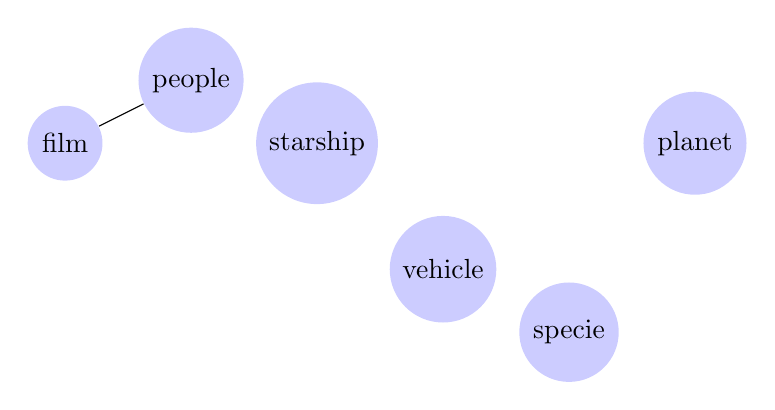
\begin{tikzpicture}
    [scale=.8,auto=left,every node/.style={circle,fill=blue!20}]
    \node (film) at (0,8)  {film};
    \node (people) at (2,9)  {people};
    \node (starship) at (4,8) {starship};
    \node (vehicle) at (6,6)  {vehicle};
    \node (specie) at (8,5)  {specie};
    \node (planet) at (10,8)  {planet};
    \foreach \from/\to in {people/film}
      \draw (\from) -- (\to);
  \end{tikzpicture}
  \caption{Entidades Starwars API (SWAPI)}
\end{figure}

\textbf{Consultas e respostas esperadas (Cliente)} \\

Para explorar bem todos os pontos de acesso da SWAPI. Foram pensadas 3 consultas de média complexidade que envolvessem pelo menos 3 das entidades descritas pela API. Para cada uma existe apenas uma resposta exata, onde é baseado nas estruturas de dados representes da API.

\begin{enumerate}
\item Qual o nome do filme no qual aparece mais personagens oriundos de um planeta deserto? R: "Revenge of the Sith"

\begin{figure}[H]
  \centering
  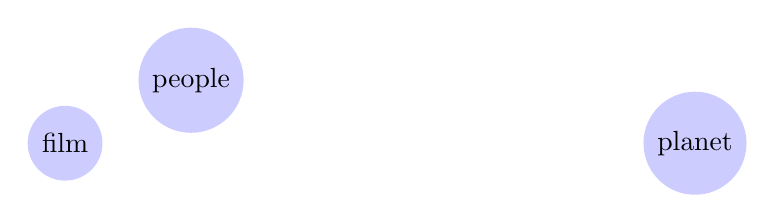
\begin{tikzpicture}
    [scale=.8,auto=left,every node/.style={circle,fill=blue!20}]
    \node (film) at (0,8)  {film};
    \node (people) at (2,9)  {people};
    \node (planet) at (10,8)  {planet};
  \end{tikzpicture}
  \caption{Entidades envolvidas na primeira pergunta}
\end{figure}

\item Qual o nome da espécie predominante entre os habitantes do planeta "Tatooine"? R: "Droid"

\begin{figure}[H]
  \centering
  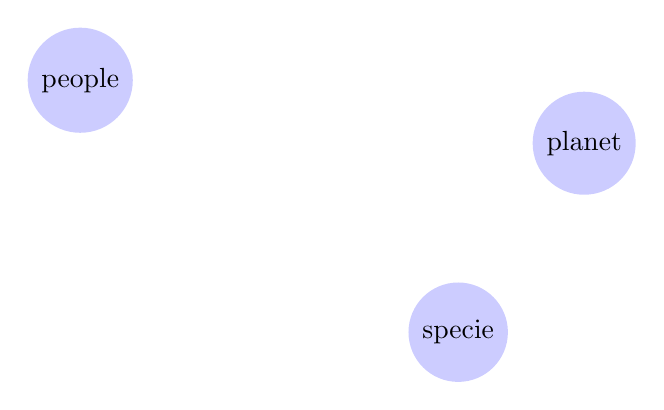
\begin{tikzpicture}
    [scale=.8,auto=left,every node/.style={circle,fill=blue!20}]
    \node (people) at (2,9)  {people};
    \node (specie) at (8,5)  {specie};
    \node (planet) at (10,8)  {planet};
  \end{tikzpicture}
  \caption{Entidades envolvidas na segunda pergunta}
\end{figure}

\item Qual o nome do personagem que mais pilota espaçonaves e veículos durante o filme "A New Hope"? R: "Chewbacca"

\begin{figure}[H]
  \centering
  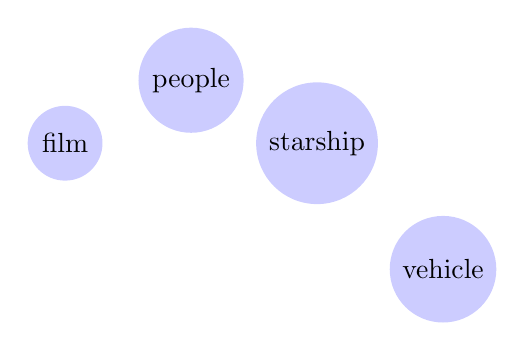
\begin{tikzpicture}
    [scale=.8,auto=left,every node/.style={circle,fill=blue!20}]
    \node (film) at (0,8)  {film};
    \node (people) at (2,9)  {people};
    \node (starship) at (4,8) {starship};
    \node (vehicle) at (6,6)  {vehicle};
  \end{tikzpicture}
  \caption{Entidades envolvidas na terceira pergunta}
\end{figure}

\end{enumerate}

\textbf{Mudanças no fluxo de dados (Servidor)} \\

Falar sobre os 3 tipos de mudanças. Primeiro é realocação, onde são pequenas mudanças no acesso. O segundo é transição, onde são considerados grandes mudanças como versionamento ou estilo de arquitetura. Por fim, o tipo de composição, onde o fluxo de dados é quebrado em diferentes serviços para separação de responsabilidades. Dizer que serão realizados 7 mudanças no fluxo de acesso da API REST (SWAPI) e comparado o impacto nos clientes.

\begin{description}[leftmargin=8em,style=nextline]
  \item[\textbf{Realocação}] 
  \begin{enumerate}
  \item Mudança no endereço de ponto de acesso.
  \item Mudança no nível de estrutura de resposta.
  \item Adição de ponto de acesso otimizado.
  \item Remoção de ponto de acesso deprecado.
  \end{enumerate}
  \item[\textbf{Transição}] 
  \begin{enumerate}
  \item[5.] Mudança de versão.
  \item[6.] Mudança no estilo de arquitetura.
  \end{enumerate}
  \item[\textbf{Composição}]
  \begin{enumerate}
  \item[7.] Mudança para micro-serviços.
  \end{enumerate}
\end{description}

Vale lembrar que nem todos os estilos de arquiteturas são vulneráveis a esses 3 tipos de mudanças. GraphQL por exemplo é desenvolvido para evitar mudanças de realocação, pois possuem apenas um acesso. Já REST, dependendo da sua implementação, está suscetível aos três. \\

\textbf{Variáveis} \\

Foram descritas treze variáveis para análise. doze delas quantitativas e uma delas qualitativa. Variáveis com o sufixo ** representam após a mudança. As variáveis que envolvem código referem-se ao código do cliente. Já o tamanho é considerado o código levado para configurar, buscar os dados e processar a resposta.

\begin{table}[H]
  \centering
  \begin{tabular}{|c|c|c|}
    \hline
    Variável & Unidade & Tipo \\
    \hline
    Tamanho do código & kb & Quantitativa \\
    \hline
    Tempo de resposta & ms & Quantitativa \\
    \hline
    Tamanho da resposta & kb & Quantitativa \\
    \hline
    Porcentagem de acerto & \% & Quantitativa \\
    \hline
    Contagem de requisição & inteiro & Quantitativa \\
    \hline
    Tempo de overhead & ms & Quantitativa \\
    \hline
    Buscou dados? ** & sim/não & Qualitativa \\
    \hline
    Tamanho do código ** & kb & Quantitativa \\
    \hline
    Tempo de resposta ** & ms & Quantitativa \\
    \hline
    Tamanho da resposta ** & kb & Quantitativa \\
    \hline
    Porcentagem de acerto ** & \% & Quantitativa \\
    \hline
    Contagem de requisição ** & inteiro & Quantitativa \\
    \hline
  	Código adicionado ** & kb & Quantitativa \\
    \hline
  	Código removido ** & kb & Quantitativa \\
    \hline
  \end{tabular}
  \caption{Variáveis de validação}
\end{table}

 
 
 
 
 
 

 


% \chapter{Resultados}

\begin{figure}[H]
  \centering
  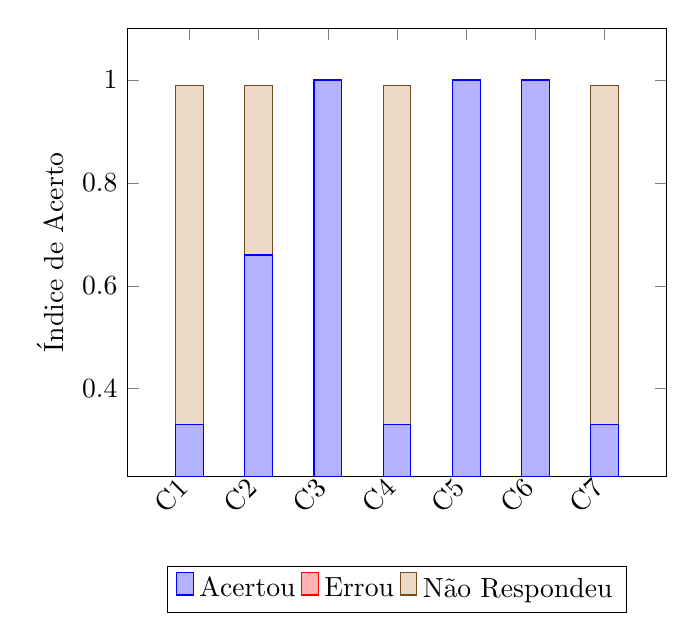
\begin{tikzpicture}
  \begin{axis}[
      ybar stacked,
      enlargelimits=0.15,
      legend style={at={(0.5,-0.20)},
        anchor=north,legend columns=-1},
      ylabel={Índice de Acerto},
      symbolic x coords={C1, C2, C3, C4, 
          C5, C6, C7},
      xtick=data,
      x tick label style={rotate=45,anchor=east},
      ]
  \addplot+[ybar] plot coordinates {(C1,0.33) (C2,0.66) 
    (C3,1) (C4,0.33) (C5,1) (C6,1) (C7,0.33)};
  \addplot+[ybar] plot coordinates {(C1,0) (C2,0) 
    (C3,0) (C4,0) (C5,0) (C6,0) (C7,0)};
  \addplot+[ybar] plot coordinates {(C1,0.66) (C2,0.33) 
    (C3,0) (C4,0.66) (C5,0) (C6,0) (C7,0.66)};
  \legend{Acertou, Errou, Não Respondeu}
  \end{axis}
  \end{tikzpicture}
  \caption{Índice de acerto sem o uso da ferramenta}
\end{figure}

\begin{figure}[H]
  \centering
  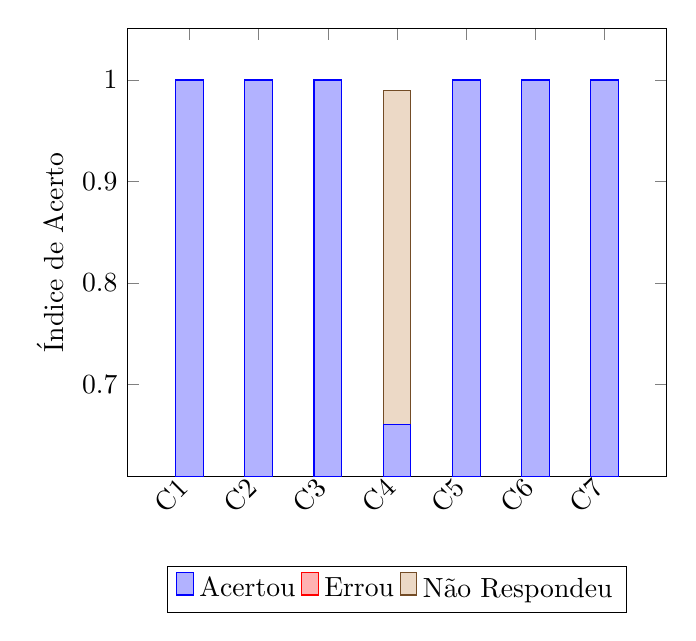
\begin{tikzpicture}
  \begin{axis}[
      ybar stacked,
      enlargelimits=0.15,
      legend style={at={(0.5,-0.20)},
        anchor=north,legend columns=-1},
      ylabel={Índice de Acerto},
      symbolic x coords={C1, C2, C3, C4, 
          C5, C6, C7},
      xtick=data,
      x tick label style={rotate=45,anchor=east},
      ]
  \addplot+[ybar] plot coordinates {(C1,1) (C2,1) 
    (C3,1) (C4,0.66) (C5,1) (C6,1) (C7,1)};
  \addplot+[ybar] plot coordinates {(C1,0) (C2,0) 
    (C3,0) (C4,0) (C5,0) (C6,0) (C7,0)};
  \addplot+[ybar] plot coordinates {(C1,0) (C2,0) 
    (C3,0) (C4,0.33) (C5,0) (C6,0) (C7,0)};
  \legend{Acertou, Errou, Não Respondeu}
  \end{axis}
  \end{tikzpicture}
  \caption{Índice de acerto com o uso da ferramenta}
\end{figure}

\begin{figure}[H]
  \centering
  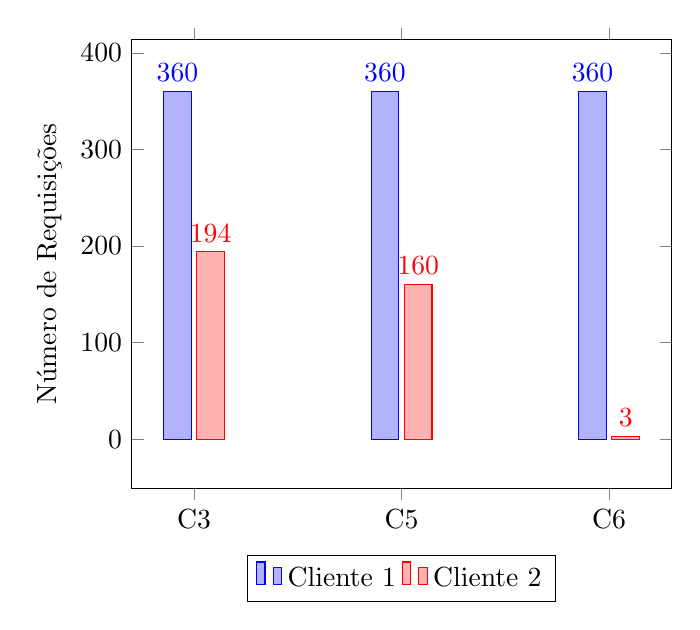
\begin{tikzpicture}
  \begin{axis}[
      ybar,
      enlargelimits=0.15,
      legend style={at={(0.5,-0.15)},
        anchor=north,legend columns=-1},
      ylabel={Número de Requisições},
      symbolic x coords={C3,C5,C6},
      xtick=data,
      nodes near coords,
      nodes near coords align={vertical},
      ]
  \addplot coordinates {(C3,360) (C5,360) (C6,360)};
  \addplot coordinates {(C3,194) (C5,160) (C6,3)};
  \legend{Cliente 1,Cliente 2}
  \end{axis}
  \end{tikzpicture}
  \caption{Comparação no número de requisições das mudanças OK}
\end{figure}

\begin{figure}[H]
  \centering
  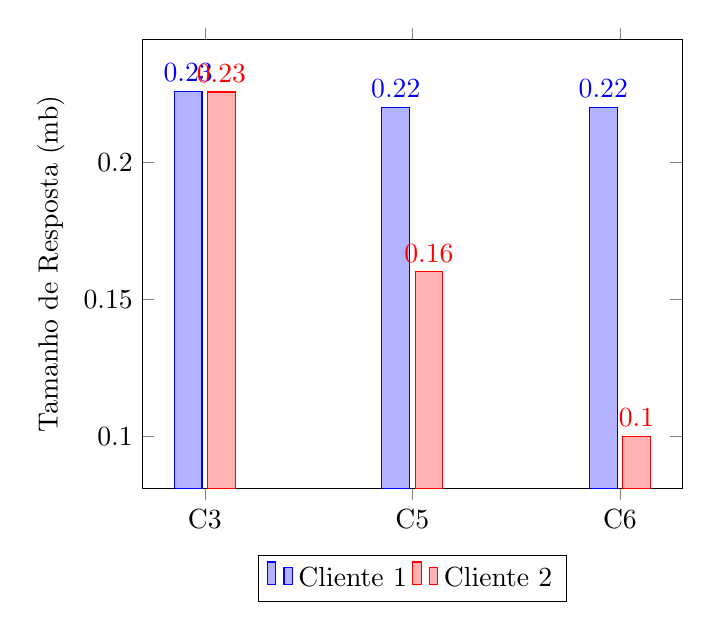
\begin{tikzpicture}
  \begin{axis}[
      ybar,
      enlargelimits=0.15,
      legend style={at={(0.5,-0.15)},
        anchor=north,legend columns=-1},
      ylabel={Tamanho de Resposta (mb)},
      symbolic x coords={C3,C5,C6},
      xtick=data,
      nodes near coords,
      nodes near coords align={vertical},
      ]
  \addplot coordinates {(C3,0.225777) (C5,0.22) (C6,0.22)};
  \addplot coordinates {(C3,0.225572) (C5,0.16) (C6,0.10)};
  \legend{Cliente 1,Cliente 2}
  \end{axis}
  \end{tikzpicture}
  \caption{Comparação no tamanho de resposta das mudanças OK}
\end{figure}

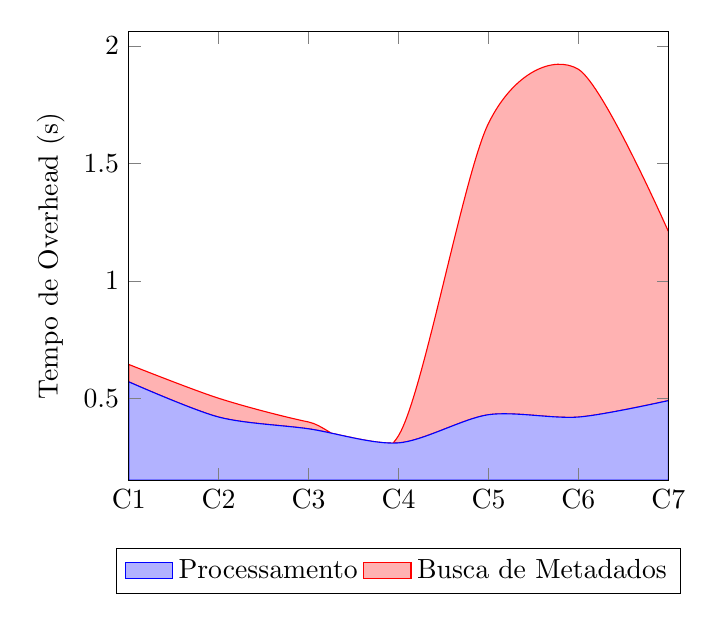
\begin{tikzpicture}
	\begin{axis}[
        ylabel={Tempo de Overhead (s)},
        legend style={at={(0.5,-0.15)},
        anchor=north,legend columns=-1},
		smooth,
		stack plots=y,
		area style,
        symbolic x coords={C1,C2,C3,C4,C5,C6,C7},
		enlarge x limits=false]
	\addplot coordinates
		{(C1,0.57) (C2,0.42) (C3,0.37) (C4,0.31) (C5,0.43) (C6,0.42) (C7,0.49)} 
		\closedcycle;
	\addplot coordinates
		{(C1,0.074) (C2,0.08) (C3,0.029) (C4,0.031) (C5,1.24) (C6,1.48) (C7,0.72)}
		\closedcycle;
    \legend{Processamento,Busca de Metadados}
	\end{axis}
\end{tikzpicture}

% \subsubsection[Sem Estado]{Sem Estado}

Como HTTP é um protocolo sem conexão (onde não há nenhuma garantia sobre qual servidor será processado e quanto tempo irá levar) cada requisição deve conter todas as informações necessarias para que um servidor entenda o que um cliente está executando. Ou seja, para ser stateless, um servidor não pode guardar informações de estado do cliente, como sessões por exemplo. \cite{Fielding2000}

Esta restrição ajuda na viabilidade, confiabilidade e escalabilidade de sistemas distribuídos. Garantem que chamadas da API não estejam vinculadas a um determinado servidor. Contudo, com base no número da diversidade de clientes, ao manter um servidor sem estado é possível perder controle no tamanho de resposta, o que pode ser um fator crucial para aplicações que dependem disso. \cite{Wildermuth2015}


\bibliographystyle{abnt-alf}
\bibliography{bibliografia/index}
\anexo
\subsubsection[Sem Estado]{Sem Estado}

Como HTTP é um protocolo sem conexão (onde não há nenhuma garantia sobre qual servidor será processado e quanto tempo irá levar) cada requisição deve conter todas as informações necessarias para que um servidor entenda o que um cliente está executando. Ou seja, para ser stateless, um servidor não pode guardar informações de estado do cliente, como sessões por exemplo. \cite{Fielding2000}

Esta restrição ajuda na viabilidade, confiabilidade e escalabilidade de sistemas distribuídos. Garantem que chamadas da API não estejam vinculadas a um determinado servidor. Contudo, com base no número da diversidade de clientes, ao manter um servidor sem estado é possível perder controle no tamanho de resposta, o que pode ser um fator crucial para aplicações que dependem disso. \cite{Wildermuth2015}

\end{document}
